\subsection{Glyph: \glyph{Equivalence}}
\label{sec:equivalence}
%The glyph \glyph{equivalence} is used to denote that all the \glyph{EPNs} linked as input are necessary to produce the output.  
The \glyph{equivalence operator} provides a mechanism to sub-class EPNs. For example, this operator allows specifying that macromolecules or nucleic acid features X\textsubscript{1}, X\textsubscript{2}, and X\textsubscript{3} are subclasses of X. This avoids the need for processes that apply to all subtypes of X to be duplicated and simplifies cases where combinatorial explosions of the number of EPNs or PNs may arise. Caution should be used with this glyph as there is the possibility that ambiguity may be introduced into a SBGN map. Examples of the correct usage of this glyph are provided in Appendix~\ref{ex_eq} together with examples of misuse along with a proposed set of guidelines for the use of this \glyph{equivalen

\begin{glyphDescription}

\glyphSboTerm
SBO:0000392 ! equivalence


\glyphIncoming Two or more \glyph{logic arcs} (\sect{logicArc}).



\glyphOutgoing
One \glyph{logic arc} (\sect{logicArc}).


\glyphContainer
An \glyph{equivalence} operator is represented by a circular shape containing the symbol ``$\Xi$'' (letter ``xi'' of the Greek alphabet).
The choice of the symbol is motivated by its use in mathematics for describing relationships as ``equivalent to'' or ``identical to''.
% 
The shape is linked to two ports, that are small arcs attached to the centres of opposite sides of the shape, as shown in \fig{equivalenceOperator}.


\glyphLabel
None.

\glyphAux
None.

\end{glyphDescription}

\begin{figure}[H]
  \centering
  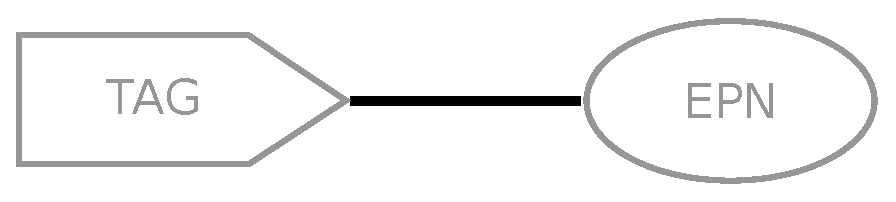
\includegraphics{images/equivalence}
  \caption{The \PD glyph for \glyph{equivalence operator}. Only two inputs are represented, but more would be allowed.}
  \label{fig:equivalenceOperator}
\end{figure}


The example of \fig{D1_1} presents the binding of different forms of TNF$\alpha$ to two receptors, TNFR1 and TNFR2.
Only membrane TNF$\alpha$ (mTNF$\alpha$) can bind to TNFR2, while both membrane TNF$\alpha$ and soluble TNF$\alpha$ (sTNF$\alpha$) can bind to TNFR1.
Binding of both forms to TNFR1 can conveniently be represented using a generic form of TNF$\alpha$, that is built using an \glyph{equivalence operator}.


\begin{figure}
\begin{center}
\includegraphics[scale=0.45]{examples/D1_1}
\end{center}
\caption{Binding of diverse forms of TNF$\alpha$ to TNF receptors.}
\label{fig:D1_1}
\end{figure}



% \begin{center}
% \scalebox{0.5}{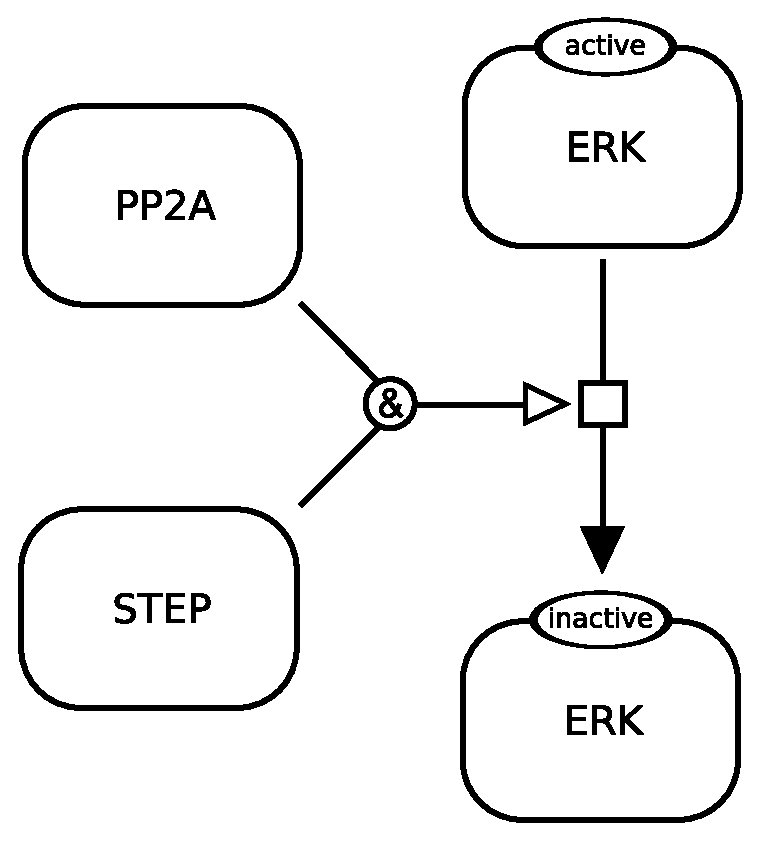
\includegraphics{images/stimulation-example1}}
% \end{center}
